\documentclass[simplex.tex]{subfiles}
% NO NEED TO INPUT PREAMBLES HERE
% packages are inherited; you can compile this on its own

\begin{document}
\subsection{ndmg}
%% Jan

In an effort to further verify that derivatives produced by the ndmg pipeline are high-quality and execution of a
given dataset within the pipeline was successful, we have expanded upon a automatically generated set of quality
control figures. In particular, we have developed the first, to our knowledge, connectome-specific graph quality
control plot. This figure, shown as the "Degree" panel in Figure~\ref{fig:ndmgqc}, considers the intra- and inter-
hemispheric connectivity of the graph, and plots the degree of each node for both same and across hemispheric
connectivity. Many real-world graphs contain node and edge attributes, but often location is not among them (or it
is used to define the edges); in connectomics, location is an important feature of each node and plays a role in its
connectivity patterns, as in whether a connection will exist within or across hemispheres of the brain. We also are
computing the mean connectome for the given dataset in this summary figure.

\begin{figure}[h!]
\begin{cframed}
\centering
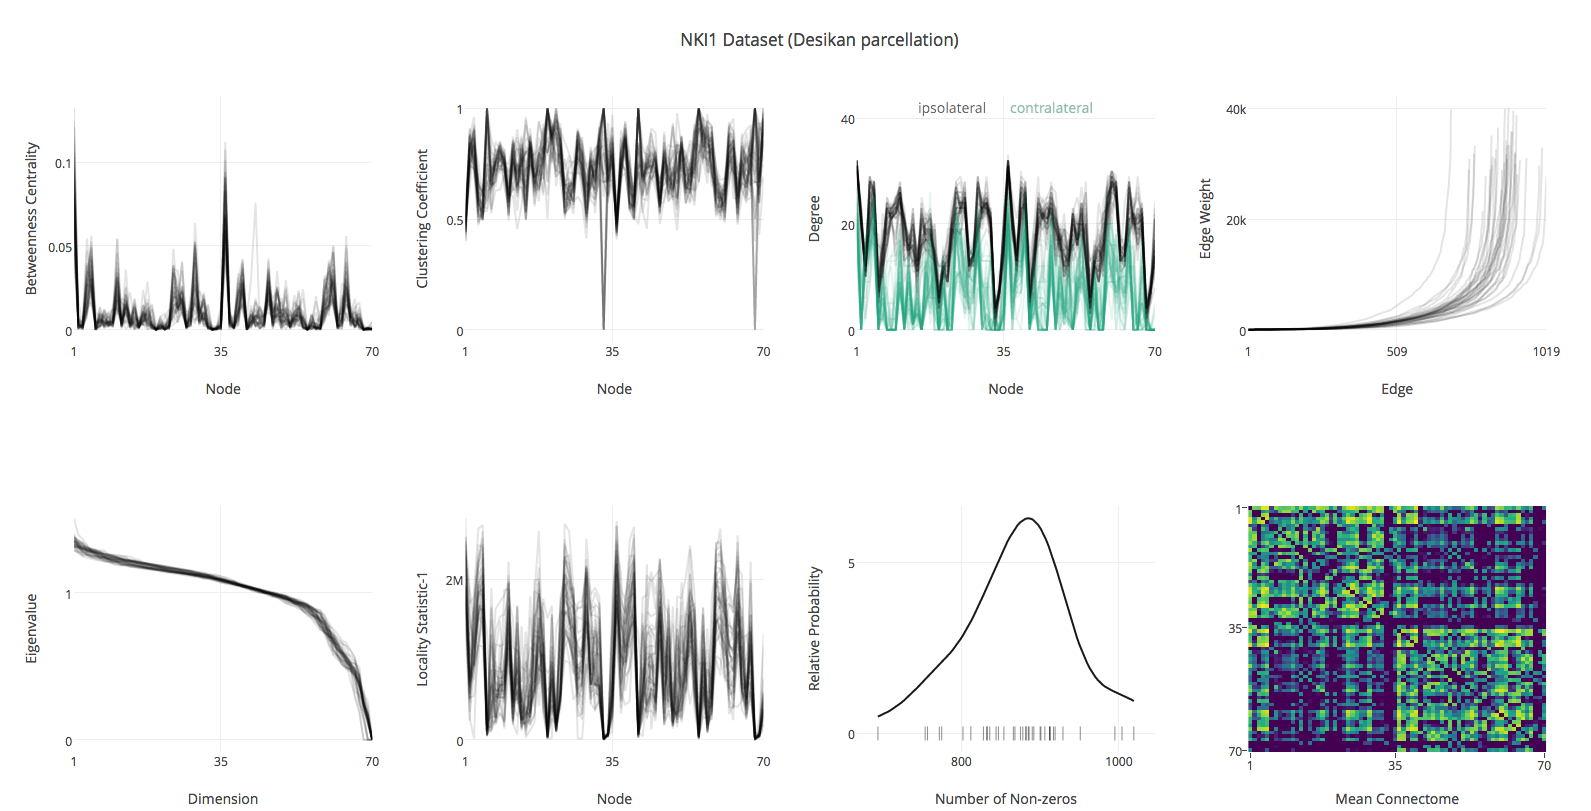
\includegraphics[width=0.95\textwidth]{../../figs/ndmgqcnew.png}
\caption{Quality Control of Connectomes}
\label{fig:ndmgqc}
\end{cframed}
\end{figure}

%% Feb
Through the use of AWS Batch, a cloud deployment script has been added to the pipeline which enables users to run the
pipeline in the cloud directly on data also stored in the cloud. This additional feature significantly lowers the
barrier to entry for use of the pipeline, and enables researchers to process and store their data without requiring
physical compute or data storage hardware or management expertise in house. Figure \ref{fig:ndmgcloud} shows an example
workflow that could be used by researchers performing a study.
\clearpage

%% March
Through use of the recently-developed cloud deployment options in ndmg, a collection of 3,000 human brain scans was
processed in a single day for under \$1,000 using our pipeline. The results are all publicly available online at our
website, \url{http://m2g.io}, and we have continued work on building a paper documenting our pipeline around this tool
and these exciting results. One such result, as shown in Figure~\ref{fig:ndmg_meanconnectome}, illustrates the mean
connectomes from a variety of datasets, and computes a multi-center mean and standard deviation connectome, as well.
This figure both illustrates the consistency of our pipeline across a wide range of data, and sheds light on properties
about the structure of the brain. Exploring these figures further, we can identify edges which are most highly variable
in the brain, and focus studies trying to understand the properties of the related regions lend themselves to such high
variability as opposed to other edges with lower variability.

\begin{figure}[h!]
\begin{cframed}[lgray]
\centering
\begin{subfigure}[h]{1\textwidth}
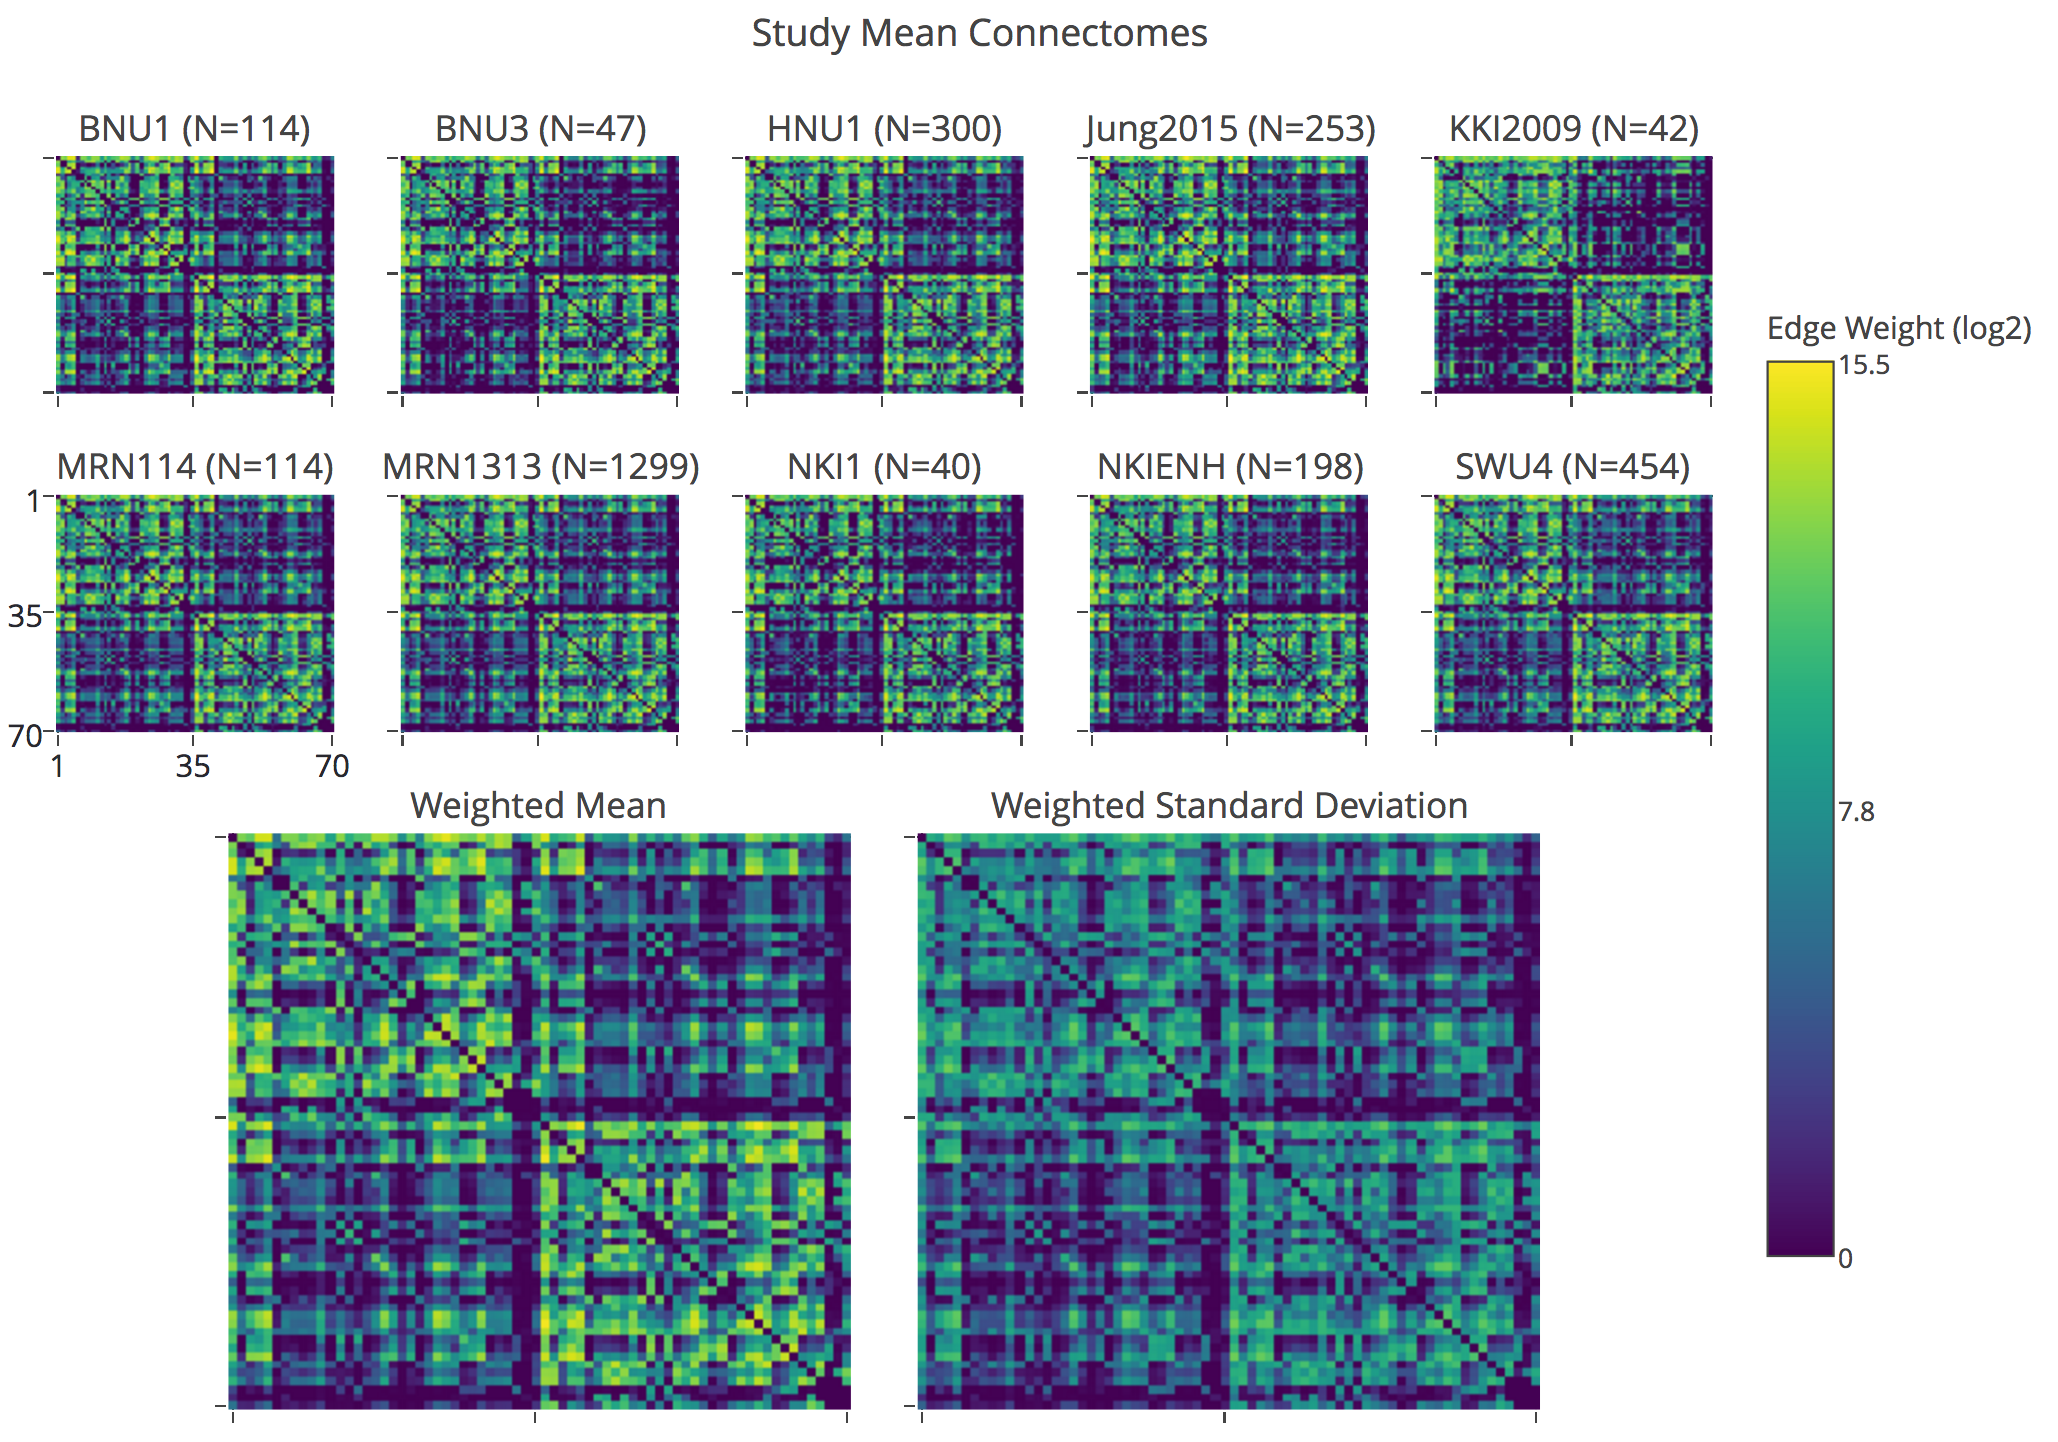
\includegraphics[width=\textwidth]{../../figs/fig_meanconnectome.png}
\end{subfigure}
\caption{\textbf{Multi-Study Mean Connectomes}. Looking at 70-nodes graphs built upon the Desikan parcellation, we have
computed the mean connectome from a variety of processed datasets. We then computed a weighted mean and standard
deviation of the mean connectomes to produce the largest known population-level connectome to-date, consisting of 2861
sessions. As expected, ipsi-lateral connectivity is consistently more dense than contra-lateral connectivity.
Similarly, the standard deviation connectome, which highlights edges that are more highly variable, shows higher
ipsi-lateral density. This suggests that not only are same-hemisphere connections more likely to occur, but they have
a higher variance than across-hemisphere connections, as well.}
\label{fig:mean}
\end{cframed}
\end{figure}

\end{document}
